\section{Attack Surface \& Models}
\todo[inline]{Does docker increase/decrease the attack surface of an host}
\todo[inline]{Does docker increase/decrease the impact/likelihood of an exploit?}
\todo[inline]{\url{https://docs.docker.com/engine/security/security/}}

Because Docker is more of an ecosystem than a single running process, it has quite a large attack surface. This attack surface consists of multiple attacker models.

\hfill

Lets take a look at the following image.

\begin{figure}[ht]
    \centering
    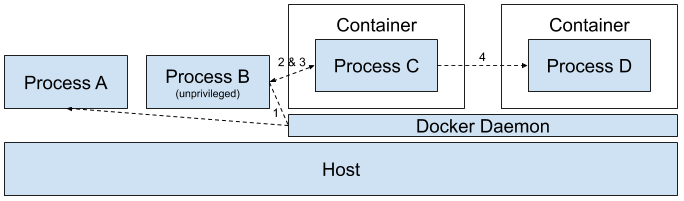
\includegraphics[width=.8\linewidth]{resources/images/attacksurfaces.png}
    \label{fig:attacksurfaces}
\end{figure}

We see four distinct processes:
\begin{enumerate}
    \item[A)] A standard (privileged) process running directly on the host.
    \item[B)] A standard unprivileged process running directly on the host.
    \item[C)] A process running in a Docker container.
    \item[D)] Similar to C.
\end{enumerate}

\hfill

We also see four distinct attacker scenarios/models:
\begin{enumerate}
    \item[1)] An unprivileged process accessing privileged data (in the image process A) using the Docker Daemon.
    \item[2)] An unprivileged process accessing data in a Docker container.
    \item[3)] A Docker container accessing data on the host (that it should not be able to access).
    \item[4)] One container accessing data in another container.
\end{enumerate}

\subsection{Container Escapes}
One of the most prominent types of vulnerability (and sometimes misconfiguration) is the possibility for a process running in a container to escape the container and access data (i.e.\ execute commands) on the host. This is scenario 3 in the \href{fig:attacksurfaces}{image above}.

\hfill

An example attack scenario would be a company that offers a PaaS (Platform as a Service) products that allows customers to run dockers on their infrastructure\footnote{This is actually quite common nowadays. All major computing providers offer such a service.}. If it is possible for the attacker to submit a Docker image that escapes the container and access the underlying infrastructure, they could access other containers or even other internal resources. That would, obviously, be a very big problem for that company.

\hfill

As noted before, because a container usages the same kernel and resources as the host; an exploit granting root can be just as devastating run inside as outside of the docker, because the target kernel and resources are the same.

It should also be noted that an exploit that allows someone to escape from a Linux \lstinline{namespace} is essentially a container escape exploit. CVE--2017--7308\cite{cve20177308} is a good example of this.

\subsection{Docker Daemon}
\todo[inline]{attacks host $\to$ container $\to$ host}
\todo[inline]{host (unprivileged) $\to$ docker}
\todo[inline]{\href{https://github.com/docker/engine/blob/v19.03.0-rc3/docs/rootless.md}{Rootless mode (Experimental)}}

\subsection{Container to Container}
\todo[inline]{attacks container $\to$ container}

\subsection{Deployment \& Development Pipelines}
One of the biggest usages of Docker is automating part of the deployment and development process.

\subsection{The impact of Docker on existing vulnerabilities}
A Docker container isolates software from the host, but does not change it. This means that vulnerabilities in software are not affected by Dockerizing that software. However, the impact of those vulnerabilities is decreased, because the vulnerability exists in a isolated environment.

If, for example, there exists a RCE (remote code execution) vulnerability in Wordpress. Running Wordpress in a Docker container does not fix the vulnerability. An attacker is still able to exploit it. But that attacker is not able to access the host system, because the exploited software is isolated from the host system because of Docker.

\subsection{Protection Mechanisms}
\todo[inline]{SELinux}
\todo[inline]{AppArmor}
\todo[inline]{Secure Computing Mode Profiles}
\todo[inline]{\url{https://github.com/genuinetools/bane}}
